\section{Amostragem e interpolação}

\begin{frame}{Amostras e amostragem}
\begin{block}{Introdução}
\begin{itemize}
	\item \textbf{Amostra} é uma observação de um sinal ou variável.
	\item O processo para a obtenção de tais observações é conhecido como \textbf{amostragem}.
\end{itemize}
\end{block}
\end{frame}

\begin{frame}{Propriedade da amostragem ou peneiramento}
\begin{block}{Amostragem ideal}
\begin{itemize}
	\item A largura das amostras são nulas.
	\item Podemos construir sinais distintos representados pela mesma sequência de amostra.
	\item \textbf{Quais as condições para que essa ambiguidade não ocorra?}
\end{itemize}
\end{block}
\centerline{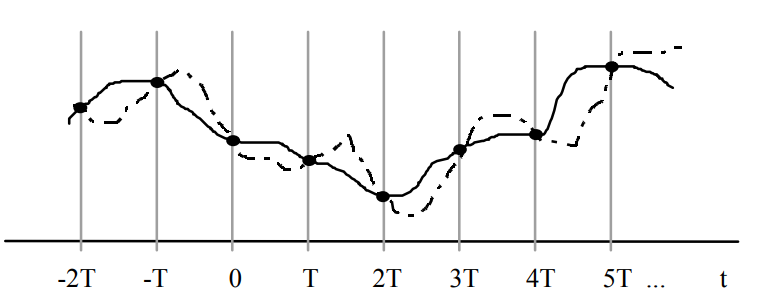
\includegraphics[width=0.9\linewidth]{Figuras/Ch02/fig3.PNG}}
\end{frame}

\begin{frame}{Propriedade da amostragem ou peneiramento}
\begin{block}{}
Sinal em tempo contínuo: $x(t)$
\end{block}
\centerline{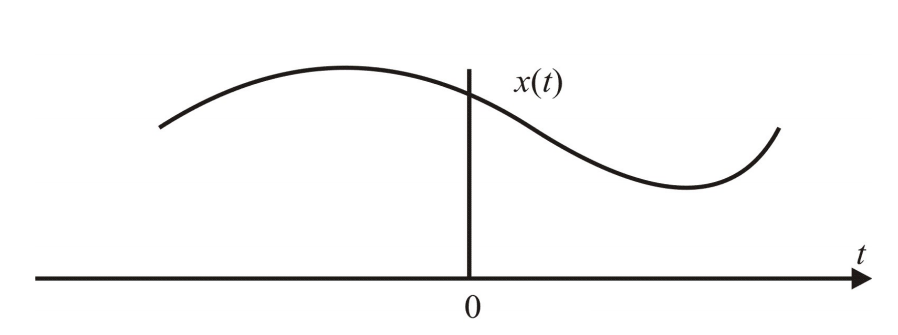
\includegraphics[width=0.9\linewidth]{Figuras/Ch02/fig4.PNG}}
\end{frame}

\begin{frame}{Propriedade da amostragem ou peneiramento}
\begin{block}{}
Função de amostragem (trem de impulsos): $p(t)$
$$\boxed{p(t) = \sum_{n=-\infty}^{\infty}\delta(t-nT)}$$
\begin{itemize}
    \item $T$ é chamado de período de amostragem e os instantes $nT$ ($n \in \mathbb{Z}$ e $nT \in \mathbb{R}$) são os instantes de amostragem e possuem unidade de tempo.
\end{itemize}
\end{block}
\centerline{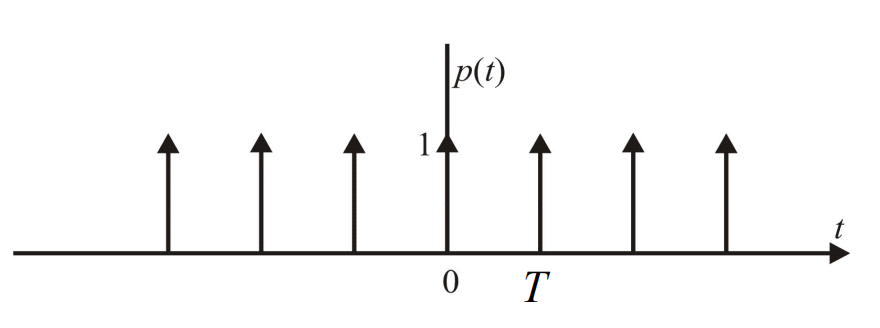
\includegraphics[width=0.8\linewidth]{Figuras/Ch02/fig5.PNG}}
\end{frame}

\begin{frame}{Propriedade da amostragem ou peneiramento}
\begin{block}{}
Sinal amostrado no tempo contínuo: $x_p(t)$
$$\boxed{x_p(t) = x(t) \cdot p(t) = \sum_{n=-\infty}^{\infty}x(nT) \cdot \delta(t-nT)}$$
\end{block}
\centerline{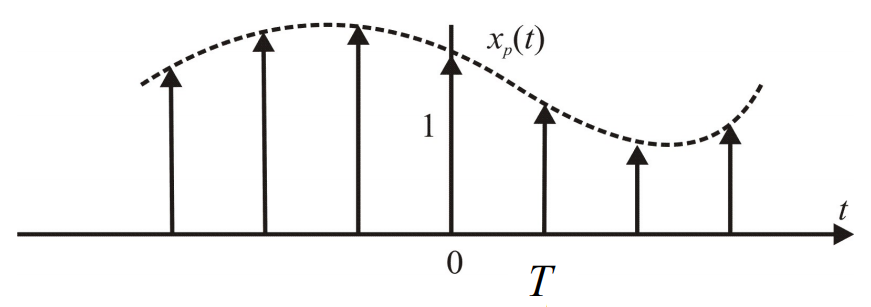
\includegraphics[width=0.7\linewidth]{Figuras/Ch02/fig6.PNG}}
\begin{block}{Propriedade de amostragem do impulso}
O produto de uma função por um impulso produz um impulso com área igual ao valor da função no instante do impulso.
\end{block}
\end{frame}

\begin{frame}{Propriedade da amostragem ou peneiramento}
\begin{block}{}
O \textbf{sinal amostrado} se obtém da multiplicação do sinal $x(t)$ com o trem de impulsos $p(t)$.
\begin{itemize}
    \item O amostrador é fechado a cada $T$ segundos. 
\end{itemize}
\end{block}
\vspace{0.3cm}
\centerline{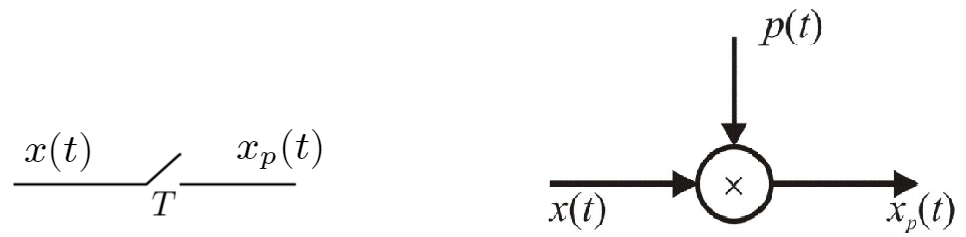
\includegraphics[width=0.9\linewidth]{Figuras/Ch02/fig7.PNG}}
\end{frame}

\begin{frame}{Propriedade da amostragem ou peneiramento}
\begin{block}{}
\begin{itemize}
    \item No entanto, $x_p(t)$ ainda é um sinal de \textbf{tempo contínuo} (embora não haja informação do sinal original $x(t)$ entre os instantes de amostragem, $x_p(t)$ é definido e tem valor -- nulo -- nestes instantes).
    \item Como transformar em um sinal de \textbf{tempo discreto}?
\end{itemize}
\begin{center}
$x_p(nT)$ ou $x_p(k)$, onde $k = n \in \mathbb{Z}$
\end{center}
\end{block}
\end{frame}

\begin{frame}{Análise da amostragem na frequência}
\begin{block}{Série de Fourier de $p(t)$}
\begin{itemize}
    \item Como $p(t)$ é um sinal periódico, este pode ser representado por meio da série de Fourier:
\end{itemize}
$$p(t) = \sum_{n=-\infty}^{\infty}c_n \text{e}^{j\omega_s nt}$$
onde
$$c_n = \dfrac{1}{T} \int_{-T/2}^{T/2} p(t) \cdot \text{e}^{-j\omega_s nt} dt = \dfrac{1}{T}$$
\end{block}
\centerline{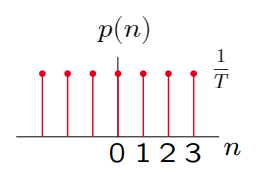
\includegraphics[width=0.4\linewidth]{Figuras/Ch02/fig17.PNG}}
\end{frame}

\begin{frame}{Análise da amostragem na frequência}
\begin{block}{Transformada de Fourier de $p(t)$}
$$P(\omega) = 2\pi \sum_{n=-\infty}^{\infty}c_n \delta(\omega - n\omega_s)$$
Deste modo:
$$P(\omega) = \dfrac{2\pi}{T} \sum_{n=-\infty}^{\infty}\delta(\omega - n\omega_s)$$
\end{block}
\vspace{0.5cm}
\centerline{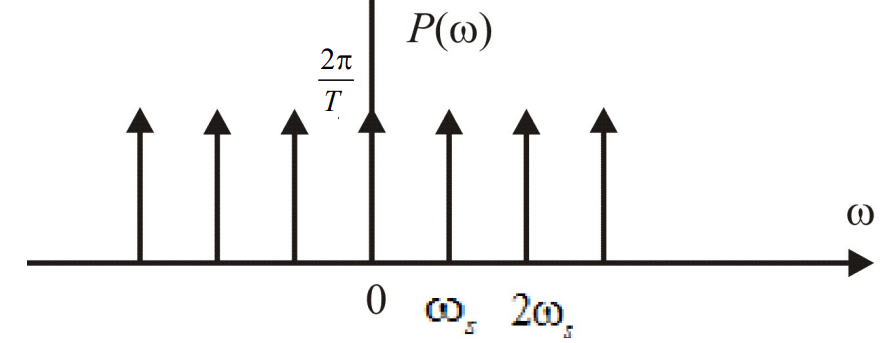
\includegraphics[width=0.6\linewidth]{Figuras/Ch02/fig8.PNG}}
\end{frame}

\begin{frame}{Teorema da amostragem}
\begin{block}{Como determinar o \textbf{espaçamento mínimo} entre as amostras para evitar \textbf{distorção}?}
Requisitos fundamentais:
\begin{itemize}
    \item $T$ constante, ou seja, amostragem uniforme.
    \item $X(\omega) = 0 \quad \forall \; \omega > \omega_M$ (banda limitada).
\end{itemize}
\end{block}
\centerline{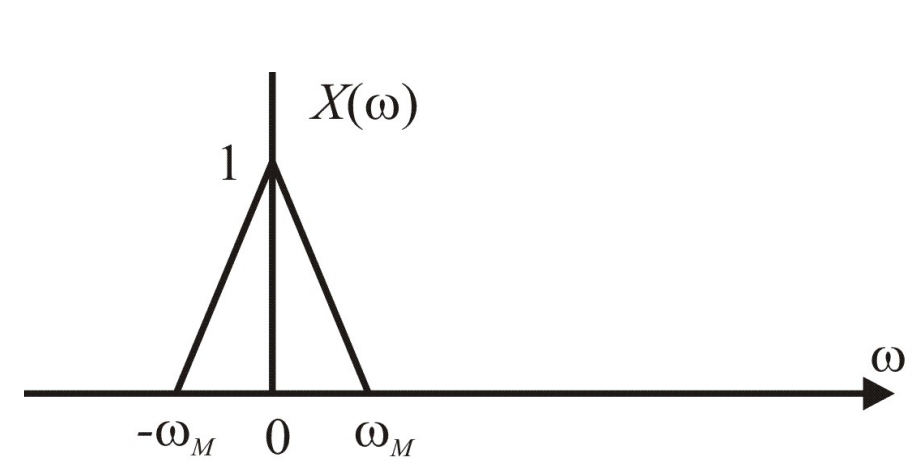
\includegraphics[width=0.6\linewidth]{Figuras/Ch02/fig9.PNG}}
\end{frame}

\begin{frame}{Teorema da amostragem}
\begin{block}{Propriedade}
$$\boxed{x_p(t) = x(t) \cdot p(t) \leftrightarrow X_p(\omega) = \dfrac{1}{2\pi}\left[X(\omega) \circledast P(\omega)\right]}$$
\begin{itemize}
    \item Ao realizar a amostragem do sinal $x(t)$, o resultado na frequência é equivalente a \textbf{replicar o espectro original} em múltiplos da frequência de amostragem $\omega_s$.
\end{itemize}
\end{block}
\end{frame}

\begin{frame}{Teorema da amostragem}
\begin{block}{Propriedade}
$$\boxed{X_p(\omega) = \dfrac{1}{T}\sum_{n=-\infty}^{\infty}X(\omega - n\omega_s)}$$
\end{block}
\centerline{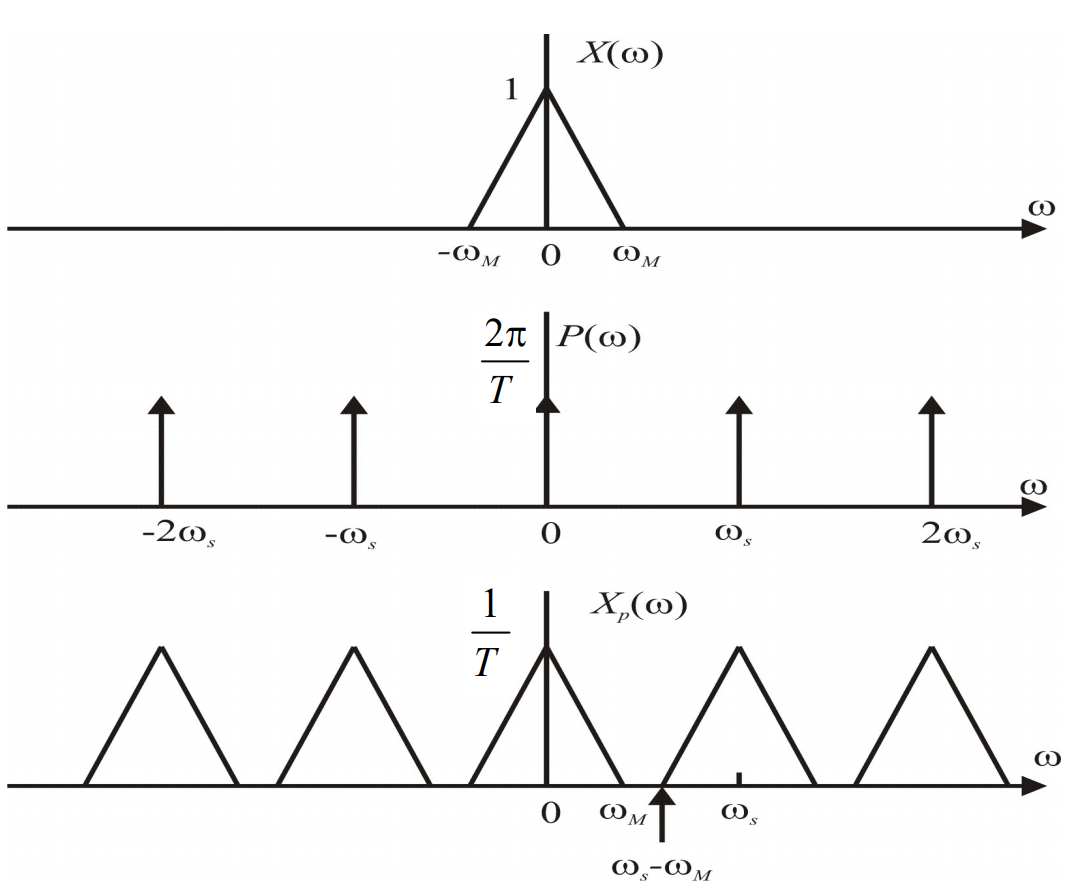
\includegraphics[width=0.5\linewidth]{Figuras/Ch02/fig10.PNG}}
\end{frame}

\begin{frame}{Teorema da amostragem}
\begin{block}{Frequência de Nyquist}
\begin{itemize}
    \item A componente não nula de maior frequência ocorre em $\omega_M$, que é a \textbf{frequência de Nyquist}. Podemos chamá-la de \textbf{frequência máxima}.
    \item Se aumentarmos $T$, as bases dos triângulos se sobrepõem. Deste modo,
\end{itemize}
$$\omega_s - \omega_M > \omega_M \implies \boxed{\omega_s > 2 \, \omega_M}$$
\end{block}
\vspace{0.5cm}
\centerline{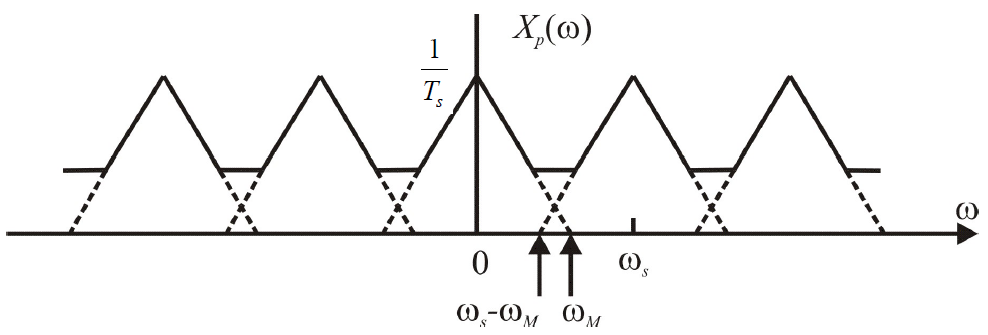
\includegraphics[width=0.9\linewidth]{Figuras/Ch02/fig11.PNG}}
\end{frame}

\begin{frame}{Teorema da amostragem}
\begin{block}{Exemplo: $f(t) = sen(t)$}
\begin{itemize}
    \item $\omega_M = 1$ rad/s. Logo, $\omega_s = 2$ rad/s.
\end{itemize}
\end{block}
\centerline{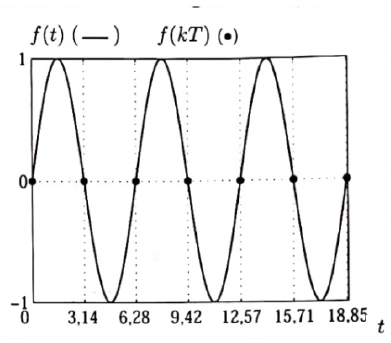
\includegraphics[width=0.4\linewidth]{Figuras/Ch02/fig12.PNG}}
\begin{block}{}
\begin{itemize}
    \item \textbf{O sinal amostrado não representa o original!} (\textit{aliasing})
    \item \textbf{Solução:} na prática é utilizado um amplo coeficiente de segurança, como $\omega_s > 10 \, \omega_M$.
\end{itemize}
\end{block}
\end{frame}

\begin{frame}{Teorema da amostragem}
\begin{block}{Filtro \textit{anti aliasing}}
\begin{itemize}
    \item Sinais \textbf{práticos} raramente são limitados em banda por conterem ruído em altas frequências. A amostragem de um sinal que não seja  limitado em banda sofrerá superposição espectral. 
    \item Na prática, para garantir que um sinal seja limitado em banda, emprega-se um filtro passa baixas (filtro \textit{anti aliasing}), cujo objetivo é fazer com que o sinal a ser amostrado não contenha componentes espectrais significativas acima de $\omega_M$.
\end{itemize}
\end{block}
\end{frame}

\begin{frame}{Interpolação}
\begin{block}{Definição}
\begin{itemize}
    \item A ideia de interpolação é conseguir \textbf{recuperar} o sinal original dadas as amostras.
    \item O efeito da amostragem no domínio da frequência é produzir réplicas da transformada de Fourier do sinal original.
\end{itemize}
\end{block}
\vspace{0.5cm}
\centerline{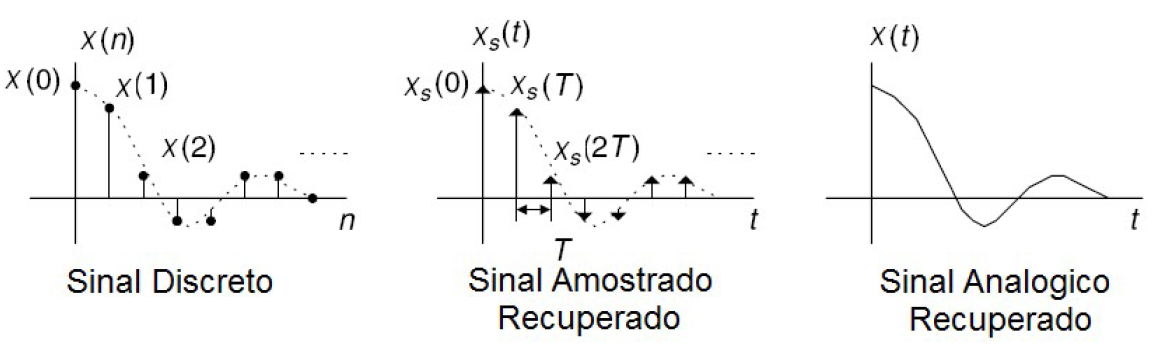
\includegraphics[width=1.1\linewidth]{Figuras/Ch02/fig13.PNG}}
\end{frame}

\begin{frame}{Interpolação}
\begin{block}{Definição}
\begin{itemize}
    \item O problema da interpolação é encontrar um sistema \textbf{interpolador} que retorne ao sinal original $x(t)$.
\end{itemize}
\end{block}
\vspace{0.5cm}
\centerline{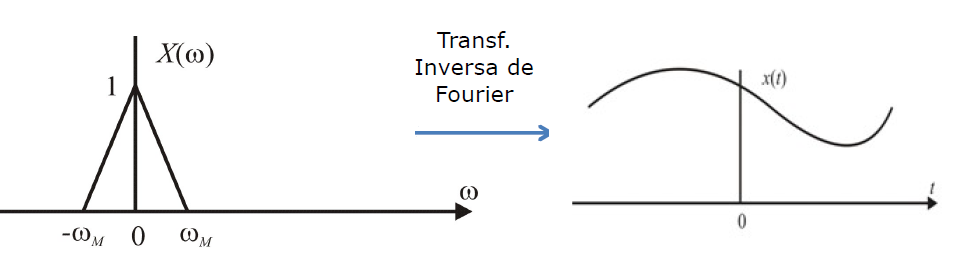
\includegraphics[width=1.1\linewidth]{Figuras/Ch02/fig14.PNG}}
\end{frame}

\begin{frame}{Interpolação}
\begin{block}{Reconstrução do sinal usando filtros analógicos}
\begin{itemize}
    \item A recuperação do espectro original $X(\omega)$ pode ser realizada utilizando um \textbf{filtro passa-baixa} ideal com frequência de corte:
\end{itemize}
$$\boxed{\omega_c = \dfrac{\omega_s}{2}}$$
\end{block}
\vspace{0.5cm}
\centerline{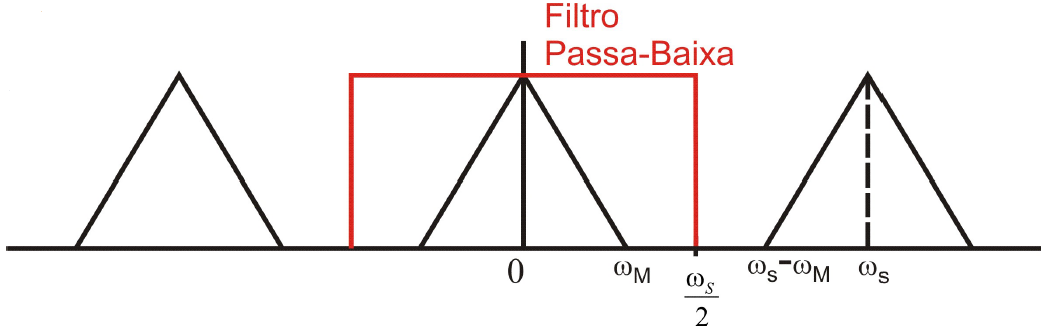
\includegraphics[width=0.9\linewidth]{Figuras/Ch02/fig15.PNG}}
\end{frame}

\begin{frame}{Interpolação}
\begin{block}{Reconstrução do sinal usando filtros analógicos}
\begin{itemize}
    \item O espectro de frequência do filtro passa-baixa ideal é:
\end{itemize}
\begin{equation*}
H(\omega) = \begin{cases}
T &\text{se $-\omega_s/2 \leq \omega \leq \omega_s/2$} \\
0 &\text{caso contrário}
\end{cases}
\end{equation*}
\begin{itemize}
    \item Se o teorema da amostragem for atendido, o sinal original  $x(t)$ pode ser recuperado a partir de $x(nT), n = 0, \pm 1, \pm 2, ...,$ construindo-se o sinal $x_p(t) = \sum_{n=-\infty}^{\infty}x(nT) \cdot \delta(t-nT)$ e fazendo-o passar  pelo filtro ideal definido acima.
\end{itemize}
\end{block}
\end{frame}

\begin{frame}{Interpolação}
\begin{block}{Reconstrução do sinal usando filtros analógicos}
\begin{itemize}
    \item A transformada inversa de Fourier resulta em:
\end{itemize}
\begin{equation*}
h(t) = \dfrac{1}{2\pi}\int_{-\infty}^{\infty} H(\omega) \text{e}^{j\omega t} d\omega = \dfrac{1}{2\pi}\int_{-\omega_s/2}^{\omega_s/2} T \text{e}^{j\omega t} d\omega
\end{equation*}
\begin{equation*}
h(t) = \dfrac{1}{2\pi} \cdot T \cdot \left[\dfrac{\text{e}^{\dfrac{j\omega_s t}{2}} - \text{e}^{\dfrac{-j\omega_s t}{2}}}{jt}\right] = \dfrac{T}{\pi t} \cdot \left[\dfrac{\text{e}^{\dfrac{j\omega_s t}{2}} - \text{e}^{\dfrac{-j\omega_s t}{2}}}{2j}\right]
\end{equation*}
\begin{equation*}
h(t) = \dfrac{T}{\pi t} \ \text{sen} \left(\dfrac{\pi t}{T}\right) =  \text{sinc} \left(\dfrac{t}{T}\right)
\end{equation*}
\end{block}
\end{frame}

\begin{frame}{Interpolação}
\begin{block}{Resposta impulsiva do interpolador}
\begin{itemize}
    \item Como a resposta em frequência do filtro ideal $H(\omega)$ é um pulso, a resposta ao impulso $h(t)$, que é a  transformada inversa de $H(\omega)$, é uma função \textbf{sinc}.
    \item \textbf{Problema}: o interpolador ideal não é \textbf{implementável}, pois a sua resposta ao impulso caracteriza um sistema \textbf{não causal}.
\end{itemize}
\end{block}
\vspace{0.5cm}
\centerline{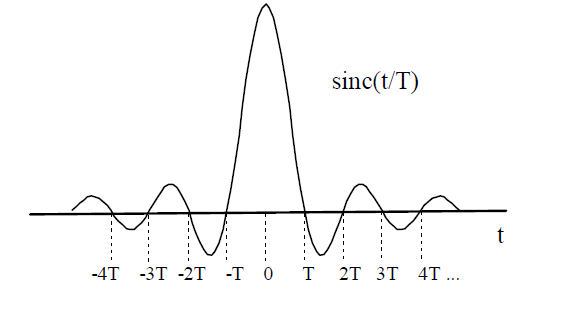
\includegraphics[width=0.6\linewidth]{Figuras/Ch02/fig16.PNG}}
\end{frame}

\begin{frame}{Interpolação}
\begin{block}{Resposta impulsiva do interpolador}
\begin{itemize}
    \item \textbf{Solução}: o que seria possível de implementar? Podemos escolher uma resposta ao impulso que receba um valor no instante $t_0$ e \textbf{segure} ao longo de $T$.
    \item O \textbf{ZOH} (\textit{zero order hold} - segurador de ordem zero) é o interpolador mais implementado na maioria dos conversores D/A.
\end{itemize}
\end{block}
\end{frame}

\begin{frame}{Conversor D/A de ordem zero}
\begin{block}{}
O conversor D/A de ordem zero aproxima os valores amostrados por um polinômio de ordem zero:
\end{block}
\begin{minipage}{0.45\linewidth}
	\centering
	\scalebox{0.8}{
		\begin{tikzpicture}
	\draw[->] (-0.2,0) -- (5,0) node[right] {$kT$};
	\draw[->] (0,-0.2) -- (0,4.5) node[above] {$u(kT)$};
	
	\draw (0,0) ++(-0.16,-0.08) node[below] {$ 0 $};
	
	\foreach \x in {1,...,4}{
		\draw (\x,0) ++(0,-0.08) node[below] {$ \x T $} -- +(0,.16);
		\node[left] at (0,\x) {$ \x $};
		\draw (0,\x) ++(-0.08,0) -- +(.16,0);
	}
	
	\draw[] plot[only marks, mark=*, mark size=1.5pt] coordinates{(0,1) (1,2) (2,4) (3,3) (4,1)};
\end{tikzpicture}}\tikzmark{A}
\end{minipage}
\hfill
\begin{minipage}{0.45\linewidth}
	\centering
	\tikzmark{B}
	\scalebox{0.8}{
		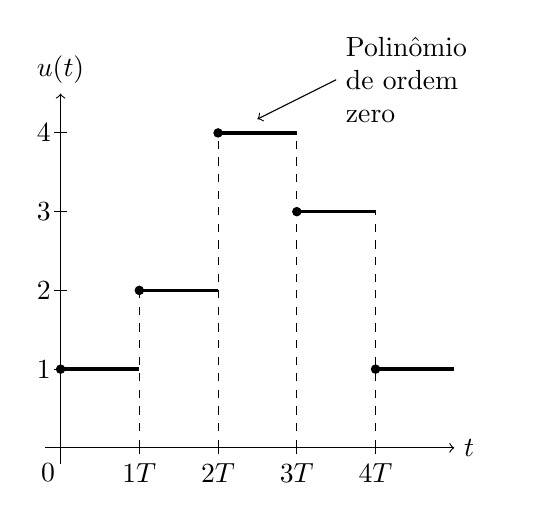
\begin{tikzpicture}
\draw[->] (-0.2,0) -- (5,0) node[right] {$t$};
\draw[->] (0,-0.2) -- (0,4.5) node[above] {$u(t)$};

\draw (0,0) ++(-0.16,-0.08) node[below] {$ 0 $};

\foreach \x in {1,...,4}{
	\draw (\x,0) ++(0,-0.08) node[below] {$ \x T $} -- +(0,.16);
	\node[left] at (0,\x) {$ \x $};
	\draw (0,\x) ++(-0.08,0) -- +(.16,0);
}

\draw[] plot[jump mark left, mark=*, mark size=1.5pt] coordinates{(0,1) (1,2) (2,4) (3,3) (4,1)};

\draw[line width=1.2pt] (0,1) -- (1,1) (1,2) -- (2,2) (2,4) -- (3,4) (3,3) -- (4,3) (4,1) -- (5,1);

\draw (4,1) -- +(0.8,0);

\draw[dashed] plot[ycomb, no marks] coordinates{(1,2) (2,4) (3,4) (4,3)};

\draw[<-] (2.5,4) ++(0,5pt) -- +(1,0.5) node[right,text width=2cm] {Polinômio de ordem zero};
\end{tikzpicture}}
\end{minipage}

\begin{tikzpicture}[overlay, remember picture]
\draw[->] (A) ++(-10pt,2cm) -- node[above] {D/A} +(1.3cm,0);
\end{tikzpicture}

\[ u(t)=u(kT)\, ,\quad kT\leqslant t<(k+1)T \]
\end{frame}


\begin{frame}{Conversor D/A de ordem zero}
\begin{minipage}{0.45\linewidth}
	\centering
	\scalebox{0.8}{
		\begin{tikzpicture}
	\draw[->] (-0.2,0) -- (5,0) node[right] {$kT$};
	\draw[->] (0,-0.2) -- (0,4.5) node[above] {$u(kT)$};
	
	\draw (0,0) ++(-0.16,-0.08) node[below] {$ 0 $};

	\foreach \x in {1,...,4}{
		\draw (\x,0) ++(0,-0.08) node[below] {$ \x T $} -- +(0,.16);
	}
	
	\draw (0,2.25) ++(-0.08,0) node[left] {$ 1 $};
	
	\draw[] plot[only marks, mark=*, mark size=1.5pt] coordinates{(0,2.25)
		(1,0) (2,0) (3,0) (4,0)};
\end{tikzpicture}}\tikzmark{A}
\end{minipage}
\hfill
\begin{minipage}{0.45\linewidth}
	\centering
	\tikzmark{B}
	\scalebox{0.8}{
		\begin{tikzpicture}
	\draw[->] (-0.2,0) -- (5,0) node[right] {$t$};
	\draw[->] (0,-0.2) -- (0,4.5) node[above] {$u(t)$};
	
	\draw (0,0) ++(-0.16,-0.08) node[below] {$ 0 $};
	
	\foreach \x in {1,...,4}{
		\draw (\x,0) ++(0,-0.08) node[below] {$ \x T $} -- +(0,.16);
	}
	
	\draw (0,2.25) ++(-0.08,0) node[left] {$ 1 $};
	
	\draw[] plot[jump mark left, mark=*, mark size=1.5pt] coordinates{(0,2.25)
		 (1,0) (2,0) (3,0) (4,0)};
	
	\draw[line width=1.2pt] (0,2.25) -- (1,2.25) (1,0) -- (4,0);
	
	\draw (0,2.25) -- +(1,0);
	
	\draw[dashed] plot[ycomb, no marks] coordinates{(1,2.25)};
\end{tikzpicture}
		}
\end{minipage}

\begin{tikzpicture}[overlay, remember picture]
\draw[->] (A) ++(-10pt,2cm) -- node[above] {D/A} +(1.3cm,0);
\end{tikzpicture}

\begin{block}{Conversor D/A de ordem zero}
	A resposta do conversor D/A pode ser dada por $ u(t)=\underbrace{d(t)}_{\text{degrau}}{}-d(t-T) $
\end{block}
\end{frame}


\begin{frame}{Conversor D/A de ordem zero}
\begin{block}{Formulação matemática}
Aplicando a transformada de Laplace em $ u(t) $:
\begin{align*}
	\mathcal{L}\{u(t)\}&=\mathcal{L}\left\lbrace d(t)-d(t-T)\right\rbrace \\
				 U(s)&=\mathcal{L}\left\lbrace d(t)\right\rbrace -\mathcal{L}\left\lbrace d(t-T)\right\rbrace \\
				 U(s)&=\dfrac{1}{s}-\dfrac{1}{s}\text{e}^{-sT}\quad \text{, logo: }\boxed{U(s)=\dfrac{1-\text{e}^{-sT}}{s}}
\end{align*}
\end{block}
\end{frame}

\begin{frame}{Conversor D/A de ordem zero}
\begin{block}{Resposta em frequência}
\begin{itemize}
    \item A resposta em frequência de um sistema linear é definida como a \textbf{transformada de Fourier} de sua resposta ao impulso.
\end{itemize}

\begin{equation*}
H(j\omega) = \int_{-\infty}^{\infty} h(t) \text{e}^{-j\omega t} \ dt
\end{equation*}

\begin{itemize}
    \item No caso do ZOH é possível tomar $s = j\omega$ porque  $u(t)$ é absolutamente integrável e, portanto,  a transformada de Fourier converge.
\end{itemize}
\end{block}
\end{frame}

\begin{frame}{Conversor D/A de ordem zero}
\begin{block}{Resposta em frequência}
\begin{itemize}
    \item Como a resposta ao impulso do ZOH tem a forma de um pulso, é de esperar que o módulo de sua transformada de Fourier seja uma função \textbf{sinc}.
\end{itemize}

\begin{equation*}
U(j\omega) = \dfrac{1 - \text{e}^{-j\omega T}}{j\omega} = \text{e}^{\dfrac{-j\omega T}{2}} \cdot \left[\dfrac{\text{e}^{\dfrac{j\omega T}{2}} - \text{e}^{\dfrac{-j\omega T}{2}}}{2j}\right] \cdot \dfrac{2T}{\omega T}
\end{equation*}
\begin{equation*}
U(j\omega) = T \text{e}^{\dfrac{-j\omega T}{2}} \cdot \dfrac{2}{\omega T} \ \text{sen} \left(\dfrac{\omega T}{2}\right) = T \text{e}^{\dfrac{-j\omega T}{2}} \cdot \text{sinc} \left(\dfrac{\omega T}{2\pi}\right)
\end{equation*}
\begin{itemize}
    \item A resposta em  frequência do ZOH é uma função sinc, com  fase adicional de $\phi = \omega T/2$, ou seja, com  \textbf{atraso puro de tempo} de $T/2$.
\end{itemize}
\end{block}
\end{frame}

\begin{frame}{Conversor D/A de ordem zero}
\begin{block}{Resposta em frequência}
\begin{itemize}
    \item A resposta em frequência do ZOH\textbf{ não é um filtro ideal}. Esse resultado já era previsto pelo fato de o ZOH ser causal. Uma consequência de  o ZOH n\textbf{ão ser um interpolador ideal} é que o sinal interpolado não será idêntico ao sinal  original, antes da amostragem.
\end{itemize}
\end{block}
\end{frame}

\begin{frame}{Conversor D/A de ordem zero}
\centerline{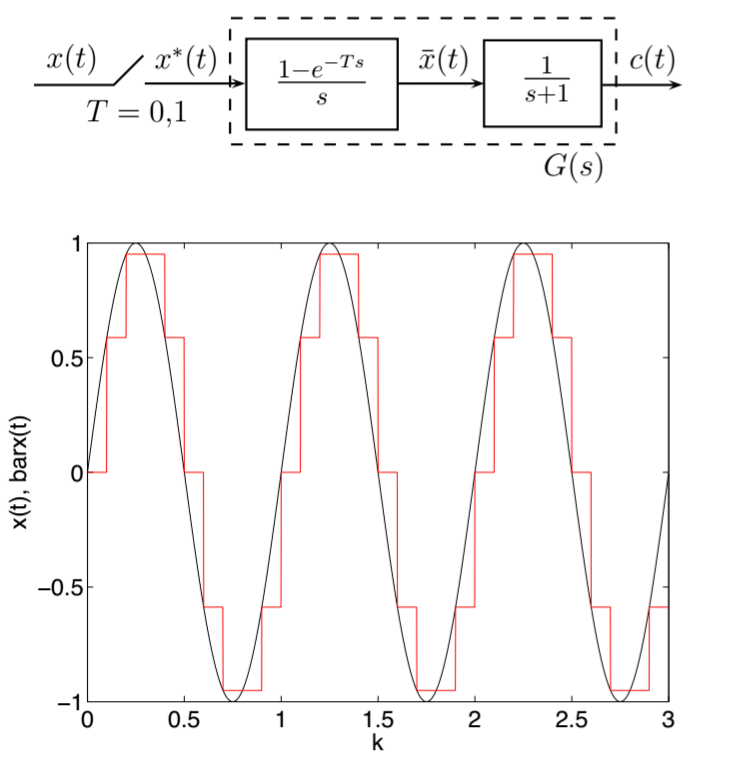
\includegraphics[width=0.65\linewidth]{Figuras/Ch02/fig20.PNG}}
\end{frame}

\frame{
\frametitle{Exercícios}
\begin{block}{}
01. Seja um sinal em tempo contínuo dado por:
$$x(t) = \text{cos}\left(30\pi t\right) + 2 \ \text{cos}\left(40\pi t\right)$$
A frequência deste sinal é dada em $rad/s$. Sabendo ainda que 1 Hz equivale a $2\pi$ rad/s, determine: (a) o valor mínimo da frequência de amostragem, $f_s$, em Hz, para que não ocorra \textit{aliasing}; (b) o período de amostragem $T$.

\vspace{0.7cm}

02. Um sinal em tempo contínuo dado por
$$x(t) = 0,5 + \text{cos}\left(2\pi t + \dfrac{\pi}{7}\right) + 3 \ \text{cos}\left(\dfrac{8\pi}{3} t\right)$$
é amostrado uniformemente com um tempo de amostragem de $T$ segundos, resultando na
sequência de tempo discreto $x(k)$. (a) Para que intervalo de $T$, $x(t)$ pode ser amostrado sem efeitos de \textit{aliasing}? (b) Seja $T = 1/4$ s. Qual é o período fundamental $N_0$ da sequência periódica resultante $x(k)$?
\end{block}
}

\frame{
\frametitle{Exercícios}
\begin{block}{}
03. Determine a transformada de Fourier de um pulso $m(t)$ centrado em  $t = 0$ mostrado na figura abaixo. Qual a diferença quando comparada com a transformada de Fourier do ZOH?
\end{block}
\centerline{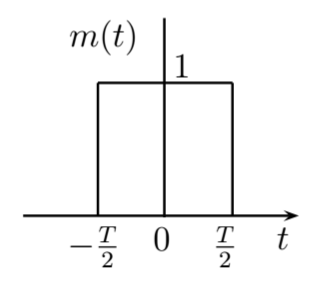
\includegraphics[width=0.4\linewidth]{Figuras/Ch02/fig19.PNG}}
}

\frame{
\frametitle{Referências e exercícios complementares}
\begin{itemize}
\item AGUIRRE, Luis A. Controle de Sistemas Amostrados, 1 ed. [s.n.], 2019.
\end{itemize}
\centering{\alert{Página 62 - \textbf{Capítulo 2}}} \\
\vspace{0.4cm}
\begin{itemize}
\item FRANKLIN, Gene F.; POWELL, J. David; WOLKMAN, Michael L. Digital Control of Dynamic Systems, 3 ed. Addison-Wesley, 1998.
\end{itemize}
\centering{\alert{Página 183 - \textbf{Capítulo 5}}} \\
}

